\documentclass[11pt,a4paper]{article}

% ---------------------------------------------------------------- packages
\usepackage[margin=25mm]{geometry}
\usepackage{amsmath,amssymb}
\usepackage{graphicx}
\usepackage{booktabs}
\usepackage{array}
\usepackage{xcolor}
\usepackage{microtype}
\usepackage[font=small,labelfont=bf]{caption}
\usepackage{tikz}
\usetikzlibrary{arrows.meta,positioning,fit,calc}
\usepackage[numbers,sort&compress]{natbib}
\usepackage[colorlinks=true,linkcolor=blue!60!black,citecolor=blue!60!black,urlcolor=blue!60!black]{hyperref}
\usepackage{url}
\usepackage{placeins}          % \FloatBarrier: keep each section's figures with its text
% let text flow under tall figures instead of giving every figure a page of its own
\renewcommand{\topfraction}{0.9}
\renewcommand{\bottomfraction}{0.6}
\renewcommand{\textfraction}{0.07}
\renewcommand{\floatpagefraction}{0.8}
\usepackage{longtable}         % appendix: the full list of validation checks

\graphicspath{{figures/}}
\emergencystretch=1.5em
\newcommand{\emgforge}{\texttt{emgforge}}
\newcommand{\dd}{\mathrm{d}}
\newcommand{\Vm}{V_{\mathrm{m}}}
\newcommand{\collab}{N.~Ezaz-Nikpay}   % harmonic-streamline fibre geometry
\newcommand{\repo}{\url{https://github.com/dhalatsis/emgforge}}
% figure, or a labelled box while the PDF does not exist yet (lets the draft compile)
\newcommand{\figorbox}[2][]{\IfFileExists{figures/#2.pdf}{\includegraphics[#1]{#2}}{\fbox{\parbox[c][55mm][c]{0.92\textwidth}{\centering\ttfamily missing figure: \detokenize{#2}}}}}

\title{\textbf{emgforge}: a first-principles-validated forward model of surface EMG, from volume-conductor lead fields to motor-unit action potentials and interference signals}

\author{Dimitrios Halatsis$^{1,*}$ \quad Noura Ezaz-Nikpay$^{2}$ \quad Pranav Mamidanna$^{1,3}$ \quad Dario Farina$^{1}$\\[6pt]
  \small $^{1}$Department of Bioengineering, Imperial College London, London, UK\\
  \small $^{2}$Department of Computing, Imperial College London, London, UK\\
  \small $^{3}$I-X Centre for AI in Science, Imperial College London, London, UK\\[4pt]
  \small $^{*}$Correspondence: \texttt{d.chalatsis22@imperial.ac.uk}. Code: \repo}
\date{Preprint --- September 2026}

\begin{document}
\maketitle

\begin{abstract}
Forward models of the electromyogram are used to explain motor-unit action potentials
(MUAPs), to test decomposition algorithms on signals with known ground truth, and to train
learning-based decoders --- but they are usually validated against each other or against
a handful of recordings, and the synthesis step that turns a lead field into a single-fibre
action potential (SFAP) is rarely checked against the physics it claims to implement. We
present \emgforge{}, an open forward model with three things that are new. First, a
synthesis method --- the line-source integral with a monopole-fitted lead field, a
second-derivative current source, a one-sided tendon window and physical time --- that we
show reproduces a closed-form line-source solution to $r = 1.0000$ and zero lag (with a
monopole-free source), and that stays usable on finite-element lead fields because the
monopole fit removes mesh ripple before the second derivative amplifies it. Second, a
tiered validation suite for forward EMG models: fifty checks with numeric criteria
drawn from the physiological literature, running from first principles through the
analytical multilayer cylinder and the finite-element conductor to MUAP phenomenology
(innervation-zone signature, end-of-fibre potential, depth decay, fat, electrode size,
inter-electrode distance, comb filtering) and interference-EMG statistics. Third, the
findings that suite produced: the spatial-frequency-domain engine that the field has used
as a reference is anti-phase and lagged relative to the line-source integral and its
propagating main lobe has inverted polarity; the width of a finite-element electrode
source shapes the lateral footprint of the lead field; and on finite-element fields the
recipe's amplitude is erratic at $\pm40\%$ while its shape and spectrum are faithful. The
model also contains an anatomical tier --- a segmented MRI forearm whose lead fields
reproduce those distributed with the NeuroDec digital twin ($r = 0.999$ over $105$
electrodes and $100$ fibres), with harmonic-streamline fibres that stay inside the muscle
by construction --- and a motoneuron-pool and
twitch layer that produces static and non-stationary interference EMG and force. Three
datasets are released with the code: a cylinder SFAP atlas, a 100-unit forearm pool with
its $5\times5$ HD-EMG MUAP tensor, and interference-EMG trials with ground-truth spikes.
\end{abstract}

% ================================================================ 1
\section{Introduction}

Forward models of the electromyogram simulate the signal an electrode records when
muscle fibres fire. They are used to understand what shapes a motor-unit action
potential, to test decomposition and estimation algorithms on signals whose ground
truth is known, and, increasingly, to generate labelled training data for
learning-based EMG decoding \citep{maksymenko2023myoelectric, ma2025conditional,
ma2024neuromotion}. The classical models are analytical: a fibre in an infinite
anisotropic medium \citep{rosenfalck1969intra, andreassen1981relationship,
nandedkar1983simulation}, a planar layered conductor \citep{farina1999compensation,
farina2001novel}, or a multilayer cylinder \citep{gootzen1991finite, blok2002three,
farina2004multilayer}. Finite-element models lift the geometric restrictions
\citep{lowery2002multiple, lowery2004volume, botelho2019anatomically} and, with
reciprocity and reusable source bases, can now be run on MRI-derived anatomy at
interactive speed \citep{maksymenko2023myoelectric}. Generative surrogates trained on
such twins \citep{ma2025conditional, ma2024neuromotion} make the output cheap and have
been validated on their own terms (a $1.8\%$ reconstruction error against the twin;
movement EMG against recordings), but a surrogate inherits its twin's synthesis step,
and the finite-element twins themselves are not distributed --- only the surrogates are.
Open models exist at the planar level \citep{petersen2019comprehensive} and as
multi-domain finite-element frameworks \citep{klotz2020modelling}; what has been missing
is an open, anatomy-capable chain whose synthesis step is checked against the physics it
implements rather than against another model.

Three of our own recent efforts depend on such a chain and motivated this one.
MUniverse \citep{mamidanna2025muniverse} benchmarks motor-unit decomposition on
synthetic, hybrid and experimental HD-EMG and needs simulation stacks whose ground truth
can be inspected; biophysical-model-informed decomposition \citep{halatsis2025bmiss}
inverts a forward model to recover spike trains and unit properties, and is only as good
as that model; and neural-operator surrogates of the lead field
\citep{halatsis2024modelling, halatsis2026neural} are trained on the finite-element fields
described here and inherit the second-derivative sensitivity discussed in
Sec.~\ref{sec:direct}.

\emgforge{} is an open, inspectable version of that chain, built on one rule: every
step must be checkable in isolation --- the lead field against an analytical model, the
synthesis integral against a closed-form solution, the MUAP features against numbers
from the physiological literature, and the whole chain against the statistics of real
interference EMG. Applying that rule is where the new results of this paper come from.
We write it plainly: what the model computes, in what order, with which parameters, and
what happened when we tested it.

The contributions are:
\begin{enumerate}
  \item \textbf{A synthesis method validated to first principles} (Sec.~\ref{sec:direct},
        \ref{sec:tierA}). \emph{Direct line-source synthesis} --- the line-source integral evaluated in space on the sampled lead field,
        with a three-monopole fit of the lead field, a second-derivative current source,
        a one-sided tendon window and physical time --- reproduces a closed-form
        line-source oracle at $r = 1.0000$ with zero lag and a monopole-free source. To our
        knowledge no published SFAP engine has been held to that test; the monopole fit is
        what makes the second-derivative integral usable on finite-element lead fields.
  \item \textbf{A tiered validation suite for forward EMG models}
        (Sec.~\ref{sec:validation}): fifty checks, each holding one measurable property
        of the chain against a literature principle with a numeric criterion, from first
        principles to interference statistics, with documented limitations kept as live
        criteria. The suite is reusable by any simulator that can produce a lead field.
  \item \textbf{Findings.} The spatial-frequency-domain engine of
        \citet{farina2001novel, farina2004multilayer}, which prior work (ours included)
        used as the shape reference, is anti-phase and lagged by $1$--$2.5$~ms relative to
        the line-source integral and its propagating main lobe has inverted polarity; the
        width of a finite-element electrode source, not the conductor, sets the lateral
        footprint of the lead field; the recipe's amplitude on finite-element fields is
        erratic at $\pm40\%$ while shape and spectrum are faithful; and an
        electrode-placement artefact in an earlier layout had been misread as a
        model property.
  \item \textbf{Anatomy from a mask}: harmonic-streamline fibre geometry
        (Sec.~\ref{sec:fibres}) that resolves contained, non-crossing fibres from a
        segmentation alone, on an MRI forearm tier whose lead fields reproduce those of
        the NeuroDec digital twin ($r = 0.999$, amplitude within $13\%$).
  \item \textbf{A complete chain and its datasets}: three interchangeable volume
        conductors behind one lead-field interface (Sec.~\ref{sec:overview}), a
        motoneuron-pool and twitch layer for static and non-stationary interference EMG
        and force (Sec.~\ref{sec:activation}), and three released datasets with ground
        truth (Sec.~\ref{sec:datasets}).
\end{enumerate}

% ================================================================ 2
\section{Overview of the pipeline}
\label{sec:overview}

Figure~\ref{fig:pipeline} shows the chain. Everything downstream of the volume
conductor is pure NumPy; only the finite-element solve needs FEniCSx
\citep{baratta2023dolfinx} and Gmsh \citep{geuzaine2009gmsh}.

\begin{figure}[tbp]
\centering
\resizebox{\textwidth}{!}{%
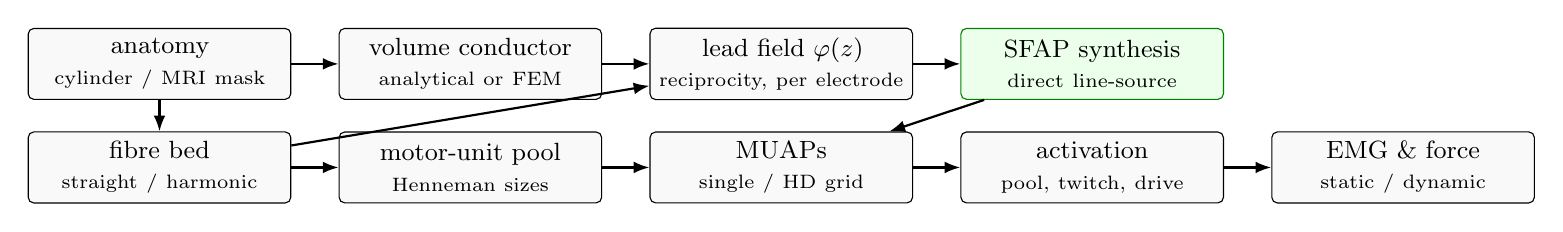
\begin{tikzpicture}[
  node distance=4mm and 6mm,
  box/.style={draw, rounded corners=2pt, minimum height=9mm, text width=31mm, align=center, font=\small, fill=gray!5},
  gold/.style={box, fill=green!8, draw=green!50!black},
  arr/.style={-{Latex[length=2mm]}, thick}]
\node[box] (anat) {anatomy\\ \scriptsize cylinder / MRI mask};
\node[box, right=of anat] (vc) {volume conductor\\ \scriptsize analytical or FEM};
\node[box, right=of vc] (lf) {lead field $\varphi(z)$\\ \scriptsize reciprocity, per electrode};
\node[gold, right=of lf] (sfap) {SFAP synthesis\\ \scriptsize direct line-source};
\node[box, below=of anat] (fib) {fibre bed\\ \scriptsize straight / harmonic};
\node[box, right=of fib] (mu) {motor-unit pool\\ \scriptsize Henneman sizes};
\node[box, right=of mu] (muap) {MUAPs\\ \scriptsize single / HD grid};
\node[box, right=of muap] (act) {activation\\ \scriptsize pool, twitch, drive};
\node[box, right=of act] (emg) {EMG \& force\\ \scriptsize static / dynamic};
\draw[arr] (anat) -- (vc); \draw[arr] (vc) -- (lf); \draw[arr] (lf) -- (sfap);
\draw[arr] (anat) -- (fib); \draw[arr] (fib) -- (mu); \draw[arr] (mu) -- (muap);
\draw[arr] (sfap) -- (muap); \draw[arr] (muap) -- (act); \draw[arr] (act) -- (emg);
\draw[arr] (fib) -- (lf);
\end{tikzpicture}}
\caption{The \emgforge{} chain. The lead field is the hinge: it is computed once per
electrode and sampled along every fibre; direct line-source synthesis turns each
fibre's $\varphi(z)$ into an SFAP; fibres are summed per motor unit, and the activation
layer turns motor-unit spike trains into interference EMG and force.}
\label{fig:pipeline}
\end{figure}

\paragraph{Reciprocity.} By the reciprocity theorem for a linear volume conductor
\citep{malmivuo1995bioelectromagnetism}, the potential at electrode $e$ due to a unit
current source at a fibre point $\mathbf{r}$ equals the potential at $\mathbf{r}$ due to
a unit current injected at $e$. So one solve with the source at the electrode gives the
\emph{lead field} $\varphi_e(\mathbf{r})$ everywhere, and sampling it along a fibre path
$\mathbf{r}(z)$ gives $\varphi_e(z)$, the weight with which membrane current at $z$
reaches the electrode. Every fibre, every motor unit and every contraction reuse the
same solve; only the number of electrodes costs finite-element work. The interior-point
reciprocity of our solver is checked directly (Sec.~\ref{sec:tierA}).

% ================================================================ 3
\section{Volume conductors and lead fields}
\label{sec:vc}

\subsection{Analytical multilayer cylinder}
The reference conductor is the four-layer cylinder of \citet{farina2004multilayer}
(bone, anisotropic muscle, fat, skin), solved in the spatial-frequency domain with
Bessel functions; \emgforge{} carries a line-by-line Python port of the original
implementation (\texttt{emgforge.analytical}). We use it in two ways: its own signal
generator produces MUAPs directly (the ``Farina generator''), and its transfer function
can be inverted to give the lead field $\varphi(z)$ along a fibre for a given electrode,
which we feed to our own synthesis engine. The geometry and conductivities are in
Table~\ref{tab:tissue}. The electrode is a disc of radius $5$~mm; the coupled grid
$\Delta z = v/f_s = 0.977$~mm (with $v = 4$~m/s, $f_s = 4096$~Hz) and $256$ samples give a
$250$~mm span along the fibre.

\subsection{Finite-element conductors}
The FEM tier solves the quasi-static conductivity equation
\begin{equation}
  \nabla\!\cdot\!\big(\boldsymbol{\sigma}(\mathbf{r})\nabla u\big) = -\,s(\mathbf{r}), \qquad
  (\boldsymbol{\sigma}\nabla u)\cdot\mathbf{n} = 0 \text{ on } \partial\Omega ,
\end{equation}
on a tetrahedral mesh with piecewise-constant tissue tensors (muscle transversely
isotropic, ratio $5$ along the fibre \citep{gielen1984electrical, rush1963resistivity};
fat, skin, bone isotropic). The source $s$ is a zero-mean Gaussian blob of width
$\sigma_{\mathrm{s}}$ centred on the electrode (its mean is subtracted so the pure-Neumann
problem is solvable), and the linear system is solved with GMRES/ILU in FEniCSx
\citep{baratta2023dolfinx}. Two families of mesh are built with Gmsh
\citep{geuzaine2009gmsh}: a \emph{parametric limb} --- layered discs (cancellous and
cortical bone, muscle, fat, skin) extruded or lofted along $z$, circular or elliptical,
optionally tapered, refined at the skin --- and the \emph{MRI forearm} (Sec.~\ref{sec:mri}).
For the cylinder used in validation the radii and conductivities are set equal to the
analytical model's (Table~\ref{tab:tissue}); the mesh has $1.03\times10^6$ cells and a
solve takes $\approx 12$~s. Figure~\ref{fig:leadfield} shows the resulting lead fields
against the analytical ones. The width of the electrode source matters more than one
might expect: with $\sigma_{\mathrm s} = 5$~mm the blob extends through the $2$~mm skin
and $3$~mm fat into the muscle, and its transverse footprint at the fibre depth is
narrower than the analytical one; a $\sigma_{\mathrm s} = 1$~mm source reproduces the
analytical transverse profile (Fig.~\ref{fig:leadfield}c).

\begin{table}[t]
\centering\small
\caption{Volume-conductor parameters. The validation cylinder uses the analytical
values in both models; the production FEM/MRI table follows \citet{gabriel1996dielectric}
at $\approx 100$~Hz.}
\label{tab:tissue}
\footnotesize\setlength{\tabcolsep}{4pt}
\begin{tabular}{lccccc>{\raggedright\arraybackslash}p{30mm}}
\toprule
 & bone & muscle $\sigma_\perp$ & muscle $\sigma_\parallel$ & fat & skin & radii (mm) \\
\midrule
analytical~\citep{farina2004multilayer} & 0.02 & 0.10 & 0.50 & 0.04 & 1.0 & 10 / 35 / 38 / 40 \\
FEM, validation cylinder & 0.02 & 0.10 & 0.50 & 0.04 & 1.0 & 9, 10 / 35 / 38 / 40; $L=240$ \\
FEM / MRI, production & 0.02$^{\dagger}$ & 0.2455 & 1.228 & 0.0379 & $4.55\times10^{-4}$ & from the segmentation \\
\bottomrule
\multicolumn{7}{p{150mm}}{$^{\dagger}$cortical; cancellous bone 0.075 S/m. The skin values differ by
$2000\times$ between the two tables: the analytical school treats skin as a thin conductive
layer ($1$~S/m), the Gabriel-based tables as dry skin ($4.6\times10^{-4}$~S/m); it is the
largest disagreement in the literature and a distinct thin skin layer changes the lateral
decay \citep{blok2002three}.}
\end{tabular}
\end{table}

\begin{figure}[tbp]
\centering
\figorbox[width=\textwidth]{fig_cylinder_leadfield}
\caption{Lead fields on the validation cylinder. (a) Cross-section with the electrode
and the fibre depths used. (b) $\varphi(z)$ along fibres 7, 13 and 20~mm below the skin:
analytical (solid) and FEM (dashed); the widths agree for deep fibres and differ for the
shallowest, where the electrode models differ (a $\varnothing10$~mm disc against a
Gaussian source that behaves as a $\varnothing5$~mm disc). (c) Transverse decay at the
fibre depth ($r=30$~mm): the FEM field around the circumference (FWHM $25$~mm; the band
is the baseline uncertainty) against the analytical peak potential for fibres displaced
around the circumference (FWHM $40$~mm); with a $\sigma_{\mathrm s}=1$~mm source the FEM
profile matches the analytical one (extra points), so the difference is the $5$~mm
electrode blob, not the conductor. (d) The FEM lead field of one electrode on the
cross-section (log scale); the dots are the fibres of (b).}
\label{fig:leadfield}
\end{figure}

\subsection{MRI forearm}
\label{sec:mri}
A labelled segmentation (muscles, radius and ulna, fat/skin) is meshed into a
tetrahedral forearm with a thin skin shell; each muscle's conductivity tensor is rotated
onto that muscle's own centreline tangent, estimated from per-slice centroids and a
smoothing spline (\texttt{sigma\_mode="centerline"}). Skin electrodes are placed on the
outer surface by ray-casting onto the mesh; the HD-EMG layout used in this paper is a
regular $5\times5$ grid with $10$~mm inter-electrode distance centred over the flexor carpi
ulnaris (FCU), rows along the arm and columns around it (measured spacing $10.2$~mm along,
$10.0$~mm across). The forearm mesh used here (subject WR, $42{,}315$ cells) builds in
$5$~s and solves in $0.6$~s per electrode; sampling $\varphi$ along the $637$ fibres of
the FCU bed takes $6$~s per electrode. A fresh solve of this model reproduces the lead
fields distributed with the NeuroDec digital twin \citep{maksymenko2023myoelectric} for
the same subject (Sec.~\ref{sec:tierMRI}).

% ================================================================ 4
\section{Direct line-source SFAP synthesis}
\label{sec:direct}
We call the production recipe \emph{direct line-source synthesis}: the line-source
integral is evaluated directly, in space, on the lead field sampled along the fibre,
rather than through the spatial-frequency route of the Farina generator described
below. Its steps are few and each has a reason.

\subsection{Line-source model}
The action potential is the Rosenfalck form $V(s) = A\,s^{3}e^{-s}$ for $s>0$ ($s$ in mm,
$A = 96$~mV) \citep{rosenfalck1969intra}, launched from the neuromuscular junction at
$z_{0}$ in both directions and cut at the tendons by a window $w(z)$ over
$[z_{0}-L_{1},\, z_{0}+L_{2}]$:
\begin{equation}
  \Vm(z,t) = V\!\big(v t - |z - z_{0}|\big), \qquad
  \Vm^{w}(z,t) = \Vm(z,t)\,w(z) ,
  \label{eq:wave}
\end{equation}
so that $t=0$ is the instant the junction fires and the wave front reaches the proximal
tendon at $L_{1}/v$ and the distal one at $L_{2}/v$. A fibre of radius $a$ and
intracellular conductivity $\sigma_{\mathrm{in}}$ injects, per unit length, the membrane
current of core-conductor theory \citep{rosenfalck1969intra, plonsey2007bioelectricity},
\begin{equation}
  i_{\mathrm m}(z,t) = \sigma_{\mathrm{in}}\,\pi a^{2}\,\frac{\partial^{2}\Vm^{w}}{\partial z^{2}} ,
  \label{eq:im}
\end{equation}
and the potential at the electrode is the lead-field-weighted sum of that current,
\begin{equation}
  \mathrm{SFAP}(t) = \int i_{\mathrm m}(z,t)\,\varphi(z)\,\dd z
  \;=\; \sigma_{\mathrm{in}}\,\pi a^{2}\int \Vm(z,t)\,w(z)\,\varphi''(z)\,\dd z ,
  \label{eq:sfap}
\end{equation}
where the second form follows by integrating by parts twice (the boundary terms vanish
because $\Vm^{w}$ has compact support) and shows that the SFAP is the inner product of
the windowed action potential with the \emph{second derivative} of the lead field.
Taking $\partial^{2}/\partial z^{2}$ of the whole windowed field, rather than of each
travelling half analytically, is what produces the three source terms that the
literature separates by hand \citep{dimitrov1998precise, kleinpenning1990equivalent}: the
two propagating tripoles, the \emph{generation} term at the cusp $|z-z_0|$, and the
\emph{end-of-fibre} terms where the window cuts the wave. These are exactly the terms
that make the source monopole-free, $\int i_{\mathrm m}\,\dd z = 0$ for all $t$
\citep{petersen2019comprehensive}; we verify this to $8\times10^{-17}$
(Sec.~\ref{sec:tierA}).

\paragraph{Units and constants.} $\varphi$ from the finite-element tier is the potential,
in volts, for a unit current ($1$~A) injected at the electrode against a uniform volume
sink (the zero-mean source of Sec.~\ref{sec:vc}; the potential is therefore defined up to
a constant, which $\varphi''$ removes). The analytical $\varphi$ is recovered from the
Farina transfer function up to an arbitrary constant, so the analytical tier is used for
shape and relative laws and absolute amplitudes are quoted only from the finite-element
tier. The engine uses $\sigma_{\mathrm{in}} = 1$~S/m and $a = 50$~$\mu$m (a $100$~$\mu$m
fibre, at the large end of the $40$--$80$~$\mu$m physiological range; amplitude scales with
$a^{2}$), so the constant $\sigma_{\mathrm{in}}\pi a^{2}$ is a scale factor rather than a
calibrated quantity and absolute microvolt values carry that caveat.

\subsection{The recipe}
Discretised, Eq.~\eqref{eq:sfap} is one matrix--vector product,
$\mathrm{SFAP} = (\mathbf{C}\,\boldsymbol{\varphi})\,\Delta z$, with $\mathbf{C}$ the
$(n_t \times n_z)$ current-source-density matrix. The steps around it, and the reason
for each, are (Fig.~\ref{fig:recipe}, Table~\ref{tab:recipe}):

\begin{enumerate}
\item \textbf{Monopole denoise of $\varphi$.} A finite-element $\varphi(z)$ carries
  mesh-scale ripple. Because the SFAP integrates $\varphi''$, that ripple is amplified
  quadratically in spatial frequency. Instead of low-passing --- which rounds the real
  peak and, as we show in Sec.~\ref{sec:tierB}, halves the spectral content --- we
  replace $\varphi$ by a least-squares fit of the form the field actually has,
  $\hat\varphi(z) = \sum_{i=1}^{3} A_i/\sqrt{d_i^{2}+(z-z_i)^{2}} + c$, a sum of three
  free-position point sources. On a clean analytical $\varphi$ the fit is a near no-op
  ($r>0.99$); on a FEM $\varphi$ it changes the field itself by at most $1.8\%$ of its
  peak but lifts the correlation of $\varphi''$ with the analytical one from $0.47$ to
  $0.91$, cuts the ripple in $\varphi''$ eighteen-fold, and takes the SFAP's jaggedness
  from $0.011$ to $0.002$ (the analytical value is $0.0018$).
\item \textbf{Edge taper.} A short cosine ramp ($5$ and $10$ samples) on the two ends of
  the sampled $\varphi$, a Gibbs guard for lead fields truncated by the sampling window.
\item \textbf{Upsampling $\times 2$} (cubic spline). The second derivative needs a finer
  grid than the raw $\varphi$ or the SFAP develops a Nyquist zigzag; $\times2$ removes
  it and $\times4$ adds nothing.
\item \textbf{Current-source density.} $\mathbf{C}$ is built from the full bidirectional
  windowed field of Eq.~\eqref{eq:wave} by two numerical $z$-derivatives.
\item \textbf{One-sided tendon window.} The window $w(z)$ is flat through the junction
  and cosine-tapered over the last $25\%$ of each semi-fibre only. A symmetric Tukey
  window would notch the junction, where the wave is born; a hard boxcar produces a
  sharp end-of-fibre spike (physically right for one fibre with a sharp tendon, and the
  choice we use when comparing to sharp-tendon oracles) which in real muscle is
  softened by tendon scatter. The taper costs $r=0.998$ against the sharp-tendon oracle.
\item \textbf{Physical time.} No centring: $t=0$ is the junction, the detector lobe of
  an electrode $\Delta z$ from the junction lands at $\Delta z/v$, the end-of-fibre
  onset at $L/v$; a $10$~ms pre-roll is prepended so a junction under the electrode is
  not pinned to the window edge.
\end{enumerate}

\begin{table}[t]
\centering\small
\caption{The direct line-source recipe (\texttt{SpatialConfig}). The cylinder tier uses
$f_s = 4096$~Hz; the MRI tier $2048$~Hz with $v = 3.3$--$4$~m/s.}
\label{tab:recipe}
\begin{tabular}{llp{72mm}}
\toprule
parameter & value & why \\
\midrule
\texttt{denoise} & monopole, 3 poles & fit the analytic form of $\varphi$; removes mesh ripple before $\varphi''$ \\
\texttt{edge\_taper\_left/right} & 5 / 10 samples & Gibbs guard at the sampling-window ends \\
\texttt{upsample\_factor} & 2 & second derivative off the Nyquist zigzag \\
\texttt{csd\_derivative} & 2 & physical current source (triphasic) \\
\texttt{fiber\_window} & one-sided, $\alpha=0.25$ & flat at the junction, tapered at the tendons \\
\texttt{center\_time / t\_start\_ms} & false / $-10$ & physical time, junction at $t=0$ \\
$v$, $f_s$, $w$ & 4 m/s, 4096 Hz, 256 & coupled grid $\Delta z = v/f_s$ \\
$\sigma_{\mathrm{in}}$, $a$ & 1, 0.05 mm & amplitude constant $\sigma_{\mathrm{in}}\pi a^2$; no $1/v$ (the IAP is fixed in space) \\
\bottomrule
\end{tabular}
\end{table}

\begin{figure}[tbp]
\centering
\figorbox[width=\textwidth]{fig_recipe_anatomy}
\caption{Anatomy of direct line-source synthesis. (a) The Rosenfalck action potential and its
first and second spatial derivatives; the second derivative is the triphasic current
source. (b) The current-source-density matrix $\mathbf{C}(z,t)$ for a fibre
$[-60, 60]$~mm with the junction at $0$: two tripoles leave the junction, the cusp at
the junction and the window edges at the tendons appear as sources; boxcar (left) and
one-sided (right) tendon windows. (c) The three fibre-end windows. (d) A finite-element
lead field raw, monopole-denoised and analytical, with their second derivatives
(normalised to the analytical peak; the colour scale in (b) is clipped at the propagating
maximum --- the tendon term is $2.7\times$ larger). (e) The SFAPs each produces: the
ripple in $\varphi''$ reaches the raw SFAP and the monopole fit removes it ($r$ against the
analytical-$\varphi$ SFAP $0.909 \to 0.929$); the remaining difference from the analytical
waveform is the FEM field's own shape at this shallow depth (Sec.~\ref{sec:tierA}), not
ripple.}
\label{fig:recipe}
\end{figure}

\subsection{The spatial-frequency engine and our port of the Farina generator}
\emgforge{} also carries a spatial-frequency-domain engine after
\citet{farina2001novel, farina2004multilayer}, in which $\varphi$ is transformed along $z$,
multiplied by the fibre-end function, the action-potential spectrum and $\mathrm{j}k_z$,
and brought back to time by a Radon section, together with a line-by-line port of the
Farina generator itself (Sec.~\ref{sec:vc}). The engine was our first production engine
and the reference the spatial engine was originally tuned against. The validation in
Sec.~\ref{sec:tierA} shows that, given the same $\varphi$, the engine does not reproduce
the line-source integral --- it is anti-phase and lagged by $0.9$--$2.6$~ms --- while its
amplitude agrees with the spatial engine's to within $5\%$; and that in the ported
generator the end-of-fibre onset leads $L/v$ by $2.5$~ms and the propagating main lobe has
the opposite sign to the textbook convention. We attribute these to the orientation and
sign conventions of the action potential in our port; the original model was verified
against limiting cases and reproduced by finite elements to $3$--$5\%$
\citep{maksymenko2023myoelectric}, and a convention difference in a port is not an error
of the model. Until that audit is done we treat the spatial recipe as the reference and
keep the other two for comparison.

\subsection{From SFAPs to a MUAP}
A \emph{fibre bed} object carries, per fibre, the sampling step, the two semi-lengths,
the junction position and the conduction velocity; a MUAP is the sum of the SFAPs of the
fibres in a motor unit, each computed from its own $\varphi(z)$ with the shared
configuration. Junction scatter, conduction-velocity scatter and tendon scatter are
therefore explicit per-fibre values rather than filters: a $5$~mm junction scatter across
$50$ fibres lengthens the MUAP from $20.0$ to $22.2$~ms and reduces its peak-to-peak to
$0.86$ of the coherent sum (Sec.~\ref{sec:tierB}), the temporal dispersion real MUAPs show.
Because time is physical, this dispersion is real and not a window artefact --- the
reason the spatial engine, and not the Fourier one, carries production.

% ================================================================ 5
\section{Fibre geometry and motor units}
\label{sec:fibres}

\subsection{Straight fibre beds}
For a parametric limb, and as the default for the MRI forearm, fibres are placed on the
muscle's cross-section at mid-length by Poisson-disk sampling at a chosen density
($4$~fibres/mm$^2$ for the FCU, which oversamples the pool: the 100-unit pool only needs
a subset) and extended as full-length paths parallel to the muscle centreline, with one
global semi-length and a junction at an atlas innervation-zone fraction ($0.305$ of the
length for the FCU). This is the classical assumption; it is simple, and it is what the
literature's cylinder models assume. Its cost is discussed in Sec.~\ref{sec:limits}.

\subsection{Harmonic-streamline fibres}
Straight, constant-depth, full-length fibres are a poor description of a real muscle
belly. \collab{} contributed a method that resolves a muscle's internal architecture from
its label mask alone: solve the masked Laplace problem $\nabla^2\phi = 0$ inside the
muscle with $\phi=0$ on the proximal cap, $\phi=1$ on the distal cap and an insulated
surface, and trace the streamlines of $\nabla\phi$ (second-order Runge--Kutta) from seeds
on the mid-belly cross-section. Streamlines are contained in the muscle and never cross
by construction. In the production model each streamline is one full-length fibre with a
single junction placed at the muscle's shared innervation zone; a quality guard rejects
tracer failures (turn per step above $15^\circ$, or a longitudinal span below $30\%$ of
the muscle). An experimental variant cuts each streamline into short in-series fibres,
each with its own junction at an atlas innervation band --- the series-fibering that
long muscles show \citep{roeleveld1997motor}; it narrows the surface field to real
motor-unit widths but is not yet validated, and is gated behind a flag. On the FCU, seeded
densely enough to match the straight bed ($0.5$~mm seed grid; the library default of
$2$~mm gives only $52$ streamlines), the harmonic bed has $827$ fibres that stay inside
the mask for $99.96\%$ of their length against $96.6\%$ for the $637$ straight fibres;
their junctions lie within $1.2$~mm (s.d.) of the shared innervation zone. The
streamlines are not all full length: the median spans $0.85$ of the muscle but a quarter
span less than $0.53$ (the straight bed spans $0.89$ throughout), a bimodal distribution
that the guard keeps because short edge fibres may be real; deciding that needs
anatomical data. With the
junction at that zone the two beds give near-identical MUAPs ($\approx0.26$~$\mu$V for a
matched unit), so the harmonic advantage at this stage is anatomical rather than
electrical (Fig.~\ref{fig:mri}). One convention to watch: the harmonic model measures its
junction fraction along the muscle's principal axis, which for the FCU points the other
way from the straight bed's fibre coordinate, so the same number places the junction at
opposite ends; Fig.~\ref{fig:mri} therefore innervates both beds on the same plane. The
released datasets use the straight bed.

\begin{figure}[tbp]
\centering
\figorbox[width=\textwidth]{fig_mri_fibres}
\caption{The MRI forearm (subject WR). (a) A segmentation slice with the FCU highlighted
and the $5\times5$ electrode grid projected. (b) The FCU fibre bed at $4$~fibres/mm$^2$:
$637$ straight Poisson fibres and $827$ harmonic streamlines (one in six drawn), both
innervated on the same plane (dotted; the atlas fraction $0.305$ of the straight fibres'
length): $84\%$ of the streamlines cross it and are innervated within $1$~mm of it; the rest
start on its far side ($z = 140$--$165$~mm) and are innervated at their nearer end, the
second cluster of dots. (c) The reciprocal lead field of one
grid electrode on a mesh slice, $\varphi - \min\varphi$ on a log scale (as in
Fig.~\ref{fig:leadfield}d). (d) $\varphi$ along three fibres $4$, $10$ and $17$~mm from the
electrode, in mV per ampere injected, with the three-monopole fit the direct recipe uses
(dashed).}
\label{fig:mri}
\end{figure}

\subsection{Motor-unit pool}
Motor units are drawn from the bed following the size principle
\citep{fuglevand1993models}: $N$ sizes log-uniform between $5$ and $400$ fibres (many
small units, few large), each unit anchored on a random bed fibre and its territory
radius grown until it contains the target number of fibres, territories allowed to
overlap; units are sorted by size so that index $i$ is recruitment order. Because the bed
is a fixed sample of the muscle ($637$ fibres for $11{,}207$ fibre slots in the 100-unit
pool), fibres are shared between units --- $18$ units per fibre on average --- which is a
coarse but consistent sampling: a fibre's SFAP is computed once and reused. A unit's MUAP
is the sum of its fibres' SFAPs; Fig.~\ref{fig:pool} shows the pool and its MUAPs. The
amplitude--size relation in Fig.~\ref{fig:pool}d is therefore a consistency check (with
shared fibres at similar depths, amplitude must scale with fibre count) rather than
evidence.

\begin{figure}[tbp]
\centering
\figorbox[width=\textwidth]{fig_mu_pool_muaps}
\caption{The 100-unit FCU pool. (a) Territories on the cross-section, colour by size
($5$--$395$ fibres, median $66$; territory radii $0.6$--$13.8$~mm), with the centre
electrode of the grid. (b) Size distribution, and recruitment threshold against
recruitment order (colour: size). (c)
Direct-method MUAPs at the centre electrode of a small, a medium and a large unit ($1.7$, $28$ and
$113$~$\mu$V; across the pool $0.7$--$160$~$\mu$V, median $24$, median duration $18$~ms).
(d) MUAP amplitude against fibre count: $p2p \propto n^{1.04}$ ($r = 0.95$), the scatter
being depth (colour); with shared fibres this is a consistency check (Sec.~\ref{sec:fibres}).}
\label{fig:pool}
\end{figure}

% ================================================================ 6
\section{Activation and interference EMG}
\label{sec:activation}

The activation layer is phenomenological, written from the equations of the
Fuglevand pool as parametrised in NeuroMotion \citep{fuglevand1993models,
ma2024neuromotion}. Given a scalar excitation $E(t)\in[0,1]$:
\begin{itemize}
  \item \emph{Recruitment}: unit $i$ has a threshold $\mathrm{RTE}_i$ spread
    exponentially with range $50$ up to $E=0.75$ for the last unit.
  \item \emph{Rate coding}: once recruited, the rate is
    $\min\big(\mathrm{PFR}_i,\ \mathrm{MFR}_i + (E-\mathrm{RTE}_i)\,s_i\big)$ with the peak rate
    falling from $40$ to $30$~pps, the minimum from $10$ to $5$~pps and the slope from $50$
    to $30$~pps per unit drive across the pool --- the onion skin
    \citep{deluca2010relationship}.
  \item \emph{Spikes}: a renewal process with Gaussian inter-spike intervals of
    coefficient of variation $1/6$, re-drawn at each discharge; units de-recruit when
    $E$ drops below threshold. A common-drive fluctuation (low-passed noise at $2$~Hz)
    can be added to $E$.
  \item \emph{Force}: each discharge adds a twitch $P_i (t/T_i)\,e^{1-t/T_i}$ with
    amplitudes spanning $100\times$ and larger units contracting faster, scaled by the
    rate-dependent fusion gain of \citet{fuglevand1993models}; the sum is normalised
    to the mean force at full excitation, so force is in \%MVC.
  \item \emph{EMG}: each spike places the unit's MUAP (single channel or on every
    electrode of the grid) and the trains sum; single- and double-differential montages
    are differences of electrodes.
  \item \emph{Non-stationary EMG}: a normalised joint angle $\theta(t)$ sets the drive
    ($0.08 + 0.42\,\theta$), scales each spike's MUAP ($1 + g_a(\theta-0.5)$; shortening
    brings fibres to the electrode) and time-warps it ($1 + g_w(\theta-0.5)$), with
    library defaults $g_a = 0.7$, $g_w = 0.18$ (the trial in Fig.~\ref{fig:hdemg}e uses
    $0.8$ and $0.22$). This is a modulation layer, not a musculoskeletal model; models of
    the geometry change itself exist \citep{mesin2006finite, mesin2011insights} and are
    the next step.
\end{itemize}
Figure~\ref{fig:hdemg} shows a unit on the grid, an interference plateau, the pool's
recruitment and rate coding, a trapezoid contraction with its force, and a movement
trial.

\begin{figure}[tbp]
\centering
\figorbox[width=\textwidth]{fig_hdemg_activation}
\caption{From motor units to signals (regular $5\times5$ grid, $10$~mm spacing). (a) The
largest unit's MUAP on the grid --- rows run along the arm, columns around it --- and,
right, the column with the largest amplitude as a waterfall offset by electrode position:
the wave walks down the column at $4.28$~m/s (dashed guide; $4.1$--$4.8$ over the pool,
set $4.0$). (b) Interference HD-EMG at a $35\%$-drive plateau ($81$ of $100$ units
active): the RMS map of the grid ($9$--$48$~$\mu$V), one row of monopolar traces and the
single-differential traces of that row at a shared scale. (c) Recruitment and rate coding of the pool. (d) A trapezoid contraction at
half drive: drive (the lead-in carries the common-drive fluctuation), spikes, EMG (plateau
RMS $73$~$\mu$V), force ($46\%$~MVC); across drives $0.1$--$1.0$ the plateau RMS is
$14$--$133$~$\mu$V and the force $7$--$100\%$~MVC. (e) A movement trial: angle and
non-stationary EMG (RMS flexed/extended $8.7$).}
\label{fig:hdemg}
\end{figure}

% ================================================================ 7
\section{Validation}
\label{sec:validation}

The suite (\texttt{scripts/validation/}, $\approx4$~min) holds one measurable property of
the chain per check against a literature principle with a numeric criterion, in four
tiers: (A) the cylinder must reproduce --- first principles, then the analytical model,
then the finite-element model, then the pipeline on each; (B) the MUAP phenomenology
the literature agrees on; (C) the statistics of interference EMG and the pool; (S) the
chain-level sanity checks that ship with the simulator. Table~\ref{tab:score} is the
scoreboard, Appendix~\ref{app:checks} lists every check with its criterion and measured
value, and the full report is in the repository (\texttt{docs/validation/}). A ``known''
flag marks a documented limitation that keeps its criterion, so it turns green when
fixed, without failing the run; ``pass / total'' counts every check. The prose below
gives the three results that matter --- the engine equals the integral, the
spatial-frequency family does not, and the finite-element amplitude and depth law are
open --- and the phenomenology as a list of measured facts.

\begin{table}[t]
\centering\small
\caption{Validation scoreboard (branch \texttt{paper/arxiv-v1}; tiers C and S run on the
released forearm pool, dataset D2). ``pass / total'' counts every check; ``known'' are
documented limitations that fail without failing the tier; the two genuine failures are
discussed in Sec.~\ref{sec:limits}. Appendix~\ref{app:checks} lists all $50$ checks.}
\label{tab:score}
\begin{tabular}{lp{58mm}ccp{42mm}}
\toprule
tier & scope & pass / total & known & fail \\
\midrule
A & cylinder: first principles, analytical, FEM, pipeline & 16 / 20 & 3 & A1.1b: FEM $\varphi''$ at mid-depth, $r=0.93$ \\
B & MUAP features vs literature & 14 / 14 & 0 & --- \\
C & interference EMG and pool & 6 / 8 & 1 & C2: no refractory floor \\
S & chain-level sanity & 8 / 8 & 0 & --- \\
\bottomrule
\end{tabular}
\end{table}

\subsection{Tier A: the cylinder must reproduce}
\label{sec:tierA}

\paragraph{First principles.} A fibre in an infinite anisotropic medium has a
closed-form lead field, $\varphi(z) \propto (\rho^{2}/\sigma_\rho + z^{2}/\sigma_z)^{-1/2}$
\citep{plonsey2007bioelectricity, rush1963resistivity}, whose second derivative is
analytic. Evaluating Eq.~\eqref{eq:sfap} in the dual form on a $0.02$~mm grid gives an
oracle with no numerical derivative of the tendon step and no volume-conductor model in
the loop. The spatial engine, given the same $\varphi$ on its $0.977$~mm grid, matches
it with $r = 1.0000$, $0.9999$, $0.9999$ and lags $0.00$, $-0.05$, $-0.05$~ms for junctions
$0$, $-20$, $-30$~mm from the electrode (Fig.~\ref{fig:first}a). This is a test of the discretisation of the integral with the same action potential --- the physics of the integral is settled --- and it is what makes the later comparisons attributable. The source is
monopole-free to $7.7\times10^{-17}$; the SFAP is invariant to the sampling rate and
step ($r>0.998$, amplitude within $0.3\%$); moving the electrode by $20$~mm delays the
propagating lobe by $4.88$~ms ($\Delta z/v = 5.00$, one sample); superposition is exact;
and changing $v$ from $4$ to $3$~m/s stretches the SFAP by $1.328$ ($4/3$) and scales its
mean frequency by $0.757$ ($3/4$) \citep{lindstrom1977interpretation}. The oracle also caught
a defect: the first version of the engine divided by $v$ once too often (a constant
inherited from the spatial-frequency formulation, where the $1/v$ belongs), so its ratio
to the oracle was exactly $1/v$ --- $0.497$ at $v = 2$, $0.249$ at $v = 4$. With the
division removed the ratio is $0.994$ at every $v$ from $2$ to $5$~m/s
(Fig.~\ref{fig:first}c); the residual $0.6\%$ is the discretisation of the $0.977$~mm grid.
The correction also dissolved a long-standing puzzle in the repository: the spatial and
Fourier engines had been pinned as disagreeing in amplitude by a ``non-constant''
$3$--$5\times$; that was the $1/v$ factor across the velocities of the reference set, and
the two engines' amplitudes now agree to $0.95 \pm 0.05$, independent of $v$. The Fourier
engine on the same $\varphi$ scores $r = -0.79$, $-0.68$, $-0.64$ at lags of $1.4$, $2.6$,
$0.9$~ms (Fig.~\ref{fig:first}b).

\begin{figure}[tbp]
\centering
\figorbox[width=\textwidth]{fig_first_principles}
\caption{First principles. (a) The closed-form line-source SFAP and the spatial engine,
three junction positions. (b) The Fourier engine against the same oracle. (c) The
engine-to-oracle amplitude ratio: $0.994$--$0.995$ at every $v$ after the correction
described in the text; the dashed $1/v$ is what the uncorrected engine gave. (d) The net source
current at every instant is zero to machine precision once the junction and end terms
are included; the propagating tripoles alone leave $39\%$.}
\label{fig:first}
\end{figure}

\paragraph{Analytical against finite-element lead fields.} Along fibres $7$--$20$~mm
below the skin the FEM $\varphi(z)$ correlates with the analytical one at
$r = 0.995$--$1.000$, and at $r=0.997$--$1.000$ for fibres $10$--$45^\circ$ off the electrode
meridian. Their widths differ for the shallowest fibres (FWHM $41$ vs $35$~mm at
$7$~mm), and comparing the second derivatives against analytical electrodes of different
radii shows the FEM Gaussian source behaves as a $5$~mm-diameter disc; at mid-depth
($13$~mm) $\varphi''$ agrees only to $r=0.93$ whatever electrode is assumed --- the one
tier-A failure. The pipeline run on FEM $\varphi$ against the pipeline run on analytical
$\varphi$ gives $r = 0.90$--$0.97$ for shallow fibres and $0.998$ for deep ones; the
Fourier route, which low-passes $\varphi$ at $\approx 32$~mm wavelength, gives $0.995$--$1.000$
at all depths, which is how earlier reports of ``$r \approx 0.99$'' were obtained.

\paragraph{Timing and symmetries.} Isolating the end-of-fibre component by subtracting
the same fibre with the tendon moved $60$~mm further, its onset lands at $10.26$ and
$15.39$~ms for $L/v = 10$ and $15$ in the pipeline (within $0.4$~ms; $0.6$~ms across a
nine-electrode array, where the threshold crossing depends on the local waveform); in the
Farina generator it leads by up to $2.5$~ms. Conduction velocity from a four-electrode
array is $3.98$~m/s (pipeline) and $3.83$~m/s (Farina) for $v=4$. Rotating the electrode by $30^\circ$ equals rotating the
fibre ($r=1.000$, peak within $1\%$); shifting it $20$~mm along the axis equals shifting the
sampling window ($r=0.996$--$0.999$, the residual being the $240$~mm mesh's end effect
\citep{lowery2002multiple});
and the lead field between two interior points is reciprocal to $1.35\%$.

\subsection{Tier B: MUAP features against the literature}
\label{sec:tierB}
Each check is run on the Farina generator (the field's reference model) and on our
pipeline, with arrays and montages built by translating the lead field
(Fig.~\ref{fig:features}, Fig.~\ref{fig:phys}):
\begin{itemize}
\item \emph{Morphology}: between the junction and the tendon the monopolar SFAP is
  $+\,-\,+$ with the main lobe negative \citep{merletti2019tutorial}. The pipeline is;
  the Farina generator's main propagating lobe is positive.
\item \emph{Conduction velocity} from a single-differential array recovers $3.13$,
  $3.98$, $4.88$~m/s for set values $3$, $4$, $5$ \citep{farina2004estimation}.
\item \emph{Innervation zone}: monopolar potentials mirror about the junction
  ($r>0.998$); the single-differential channel over it is $4\%$ of the maximum and the
  channels either side are mirror images of opposite sign ($r<-0.998$)
  \citep{masuda1985position}.
\item \emph{End of fibre}: the same onset on every electrode ($0.00$~ms spread); its
  ratio to the propagating part grows monotonically with depth ($0.02$ at $7$~mm to
  $0.20$ at $20$~mm) and is suppressed mono $>$ SD $>$ DD ($0.053$, $0.014$, $0.004$)
  \citep{arabadzhiev2013peculiarities, roeleveld1998motor}.
\item \emph{Depth}: peak-to-peak amplitude is a power law in depth over $7$--$25$~mm
  ($R^{2}>0.98$), exponent $2.9$ monopolar and $3.5$ single-differential
  \citep{roeleveld1997motor, fuglevand1992detection}.
\item \emph{Fat}: RMS retained at $3/9/18$~mm of fat is $0.50/0.23/0.12$ against the
  finite-element curve $0.69/0.20/0.10$ of \citet{kuiken2003effect}; mean frequency falls;
  the FEM tier attenuates like the analytical one within $30\%$ once $\varphi$ is
  smoothed.
\item \emph{Electrode and montage}: amplitude and mean frequency fall with electrode
  radius; a $5$~mm disc is $-2.8$~dB at $100$~cycles/m \citep{merletti2019tutorial};
  single-differential amplitude doubles from IED $2.5$ to $5$~mm and saturates beyond
  $10$~mm; with a single travelling wave, the two electrodes of a bipolar pair see
  shift-copies to $2.2\times10^{-3}$ ($1.4\times10^{-3}$ without the monopole fit), so the montage is the textbook comb filter with
  nulls at $n\,v/\mathrm{IED}$ \citep{lindstrom1977interpretation, lynn1978influence}.
\item \emph{Anisotropy} elongates the lead field along the fibres by exactly $\sqrt{5}$ in
  the infinite medium and by $1.5$ in the layered cylinder.
\item \emph{Linearity}: $50$ identical fibres give $50\times$ the SFAP to $10^{-15}$.
\end{itemize}

\begin{figure}[tbp]
\centering
\figorbox[width=\textwidth]{fig_physical_time}
\caption{Physical time on a finite-element lead field (fibre 10~mm deep, tendons at
$\pm60$~mm, $v = 4$~m/s). (a) Monopolar SFAPs along a nine-electrode array with hard
tendons: the propagating lobe walks at $|z|/v$ (a fit gives $4.04$~m/s; the guide is drawn
at $|z|/v + 1.0$~ms because the negative phase trails the wave front by the action
potential's rise) while the end-of-fibre potential starts at $15.4$--$15.6$~ms on every
channel ($L/v = 15$~ms; spread $0.24$~ms). (b) The single-differential montage vanishes and reverses at the innervation
zone. (c) The same array with the one-sided tendon window of the direct recipe: the
end-of-fibre potential falls from $0.16$ to $0.10$ of the propagating amplitude.}
\label{fig:phys}
\end{figure}

\begin{figure}[tbp]
\centering
\figorbox[width=\textwidth]{fig_validation_features}
\caption{MUAP features against the literature (fibre $10$~mm below the skin unless
stated; $v = 4$~m/s). (a) Depth law of the peak-to-peak amplitude (log--log) for the
pipeline (monopolar and single-differential), the Farina generator and the FEM pipeline,
with fitted exponents. (b) RMS retained against subcutaneous fat thickness, analytical
model against the finite-element points of \citet{kuiken2003effect}; FEM pipeline
(direct and Butterworth-smoothed) and Farina generator at $2$--$8$~mm, each relative to
its thinnest case. (c) End-of-fibre to propagating amplitude ratio against depth
(junction $20$~mm and near tendon $40$~mm from the electrode). (d) Conduction velocity
recovered from a four-channel single-differential array against the set value.
(e) The monopolar and single-differential array across the innervation zone (IED
$10$~mm). (f) Transverse spread of monopolar and single-differential amplitude for a
fibre $15$~mm deep.}
\label{fig:features}
\end{figure}

\subsection{Tier C and S: interference EMG and the chain}
These tiers run on the released forearm pool (Sec.~\ref{sec:datasets}). The pool's rates
lie in $5$--$40$~pps with the onion-skin ordering ($\rho = -0.98$ between threshold and
rate); inter-spike-interval variability is $0.16$; thresholds are right-skewed and
twitches span $95\times$; the amplitude distribution is super-Gaussian at low drive
(kurtosis $5.6$ at $5\%$) and Gaussian at high ($2.9$--$3.1$ at $50$--$90\%$), with ARV/RMS
$0.77$--$0.79$, between the Laplacian and Gaussian values \citep{clancy1999probability,
nazarpour2013note}; the RMS at half maximal force is $0.56$ of that at maximal force,
inside the linear-to-quadratic band of \citet{lawrence1983myoelectric}; the median
frequency at moderate drive is $77$~Hz (mean $81$~Hz); larger units give larger MUAPs
($\rho = 0.98$). The chain-level checks pass: orderly recruitment, onion skin, EMG rising
with drive, force monotone and calibrated to $100\%$~MVC at full drive, conduction
velocity $4.33$~m/s read off the HD grid ($4.1$--$4.9$ over all $100$ units, $10$~mm
inter-electrode distance) for a set $4.0$~m/s --- the $8$--$24\%$ overestimate is the
apparent velocity $v/\cos\theta$ of fibres running $5$--$25^\circ$ to the grid columns
(the same estimator recovers $3.98$ on the cylinder, and inclination bias of this size is
documented \citep{mesin2007estimation}); the check's criterion is the physiological band
--- a localised MUAP footprint (peak/mean RMS $2.2$), an $8.7\times$ amplitude
modulation across a movement, and a MUAP scale inside the physiological band (median
peak-to-peak $23.6$~$\mu$V, range $0.7$--$160$~$\mu$V, median duration $18$~ms, against
tens to hundreds of microvolts and $5$--$20$~ms \citep{merletti2019tutorial}). Amplitude
cancellation is flagged ($68\%$ already at $20\%$ drive against $\approx33\%$ in
\citet{keenan2005influence}); see Sec.~\ref{sec:limits}.

\subsection{MRI tier}
\label{sec:tierMRI}
The NeuroDec digital twin \citep{maksymenko2023myoelectric} distributed, for subject WR,
the reciprocal lead field of each of its $105$ skin electrodes sampled along $100$ fibre
paths. Re-solving the same mesh with our solver and sampling the same paths
(\texttt{scripts/validation/mri\_neurodec\_check.py}; artefact
\texttt{docs/validation/neurodec\_wr.json}) gives a signed correlation of $0.9994$ on
average ($0.9989$--$0.9999$ over the $105$ electrodes) and an amplitude ratio of $1.13$
(median; $1.03$--$1.23$), i.e.\ the same field up to a $13\%$ scale that we attribute to
the source normalisation and skin shell of the two solvers --- the volume conductor is the
same physics on the same anatomy. On that anatomy the harmonic fibres are contained in
the muscle mask for $99.96\%$ of their length ($96.6\%$ for straight fibres). A mesh
refinement study of the $42{,}315$-cell forearm mesh against a finer one has not been
done and is listed in Sec.~\ref{sec:limits}.

% ================================================================ 8
\section{Released datasets}
\label{sec:datasets}
Three datasets are generated by scripts in \texttt{paper/figures/} and described by
manifests in \texttt{paper/datasets/} (Table~\ref{tab:data}). They are meant as
reference material: every array can be regenerated from the repository.

\begin{table}[t]
\centering\small
\caption{Datasets released with the paper (float32, NumPy \texttt{.npz} with a JSON
manifest each; $8$~MB in total).}
\label{tab:data}
\begin{tabular}{lp{86mm}r}
\toprule
name & contents & size \\
\midrule
\texttt{cylinder\_sfap\_atlas} & analytical and FEM lead fields and direct-method SFAPs on the validation cylinder for $6$ depths $\times$ $5$ angles $\times$ $3$ junction offsets $\times$ $9$ electrode positions ($1620$ SFAPs), with the Farina-generator MUAP of each case & 1.6~MB \\
\texttt{forearm\_fcu\_mu\_pool} & the 100-unit FCU pool (fibre paths, fibre indices, sizes, territories, activation parameters), direct-method MUAPs at the centre electrode and the full $(100, 25, 256)$ HD-grid MUAP tensor, electrode positions, configuration & 2.4~MB \\
\texttt{interference\_emg\_trials} & trapezoid contractions at six drive levels ($0.1$--$1.0$): drive, spike trains, single-channel and $25$-channel EMG, force; one movement trial & 4.1~MB \\
\bottomrule
\end{tabular}
\end{table}

% ================================================================ 9
\section{Limitations and open items}
\label{sec:limits}
We list these in the order we would fix them.
\begin{enumerate}
\item \textbf{Conduction velocity and amplitude.} With the constant corrected, the
  engine's amplitude is independent of $v$ because its action potential is fixed in
  space. Physiologically the action potential is fixed in \emph{time} and a faster fibre
  carries a longer wave, which is why single-fibre amplitude falls with conduction
  velocity \citep{nandedkar1983simulation}; reproducing that requires stretching the
  action potential in space with $v$, a modelling choice we have not yet made.
\item \textbf{Fourier engine.} Given a lead field, it is anti-phase and lagged relative
  to the line-source integral, and its end-of-fibre onset is early. We suspect the
  orientation and sign conventions of the action potential in the Radon formulation
  (\texttt{V2 = -flip(...)}); until audited it should not be used as an oracle.
\item \textbf{FEM lead-field fidelity for the recipe.} On finite-element $\varphi$ the
  direct-method SFAP amplitude is erratic at $\pm40\%$ across depth: the recipe integrates
  $\varphi''$ faithfully down to $\approx8$~mm wavelengths, where FEM $\varphi$ carries
  mesh structure that the three-pole fit does not remove (five or seven poles do not
  either). Low-passing $\varphi$ makes amplitudes smooth but halves the SFAP's mean
  frequency ($46$ vs $112$~Hz direct, $91$~Hz analytical). A finer mesh around the fibre
  band, or a smoothing-free local estimate of $\varphi''$, is the fix. Until then FEM
  amplitude laws should be read through the smoothed route; shape, timing and spectrum
  can be read from the direct one.
\item \textbf{Depth law.} The FEM cylinder decays $\approx30\%$ slower with depth than the
  analytical one over $7$--$20$~mm, whatever the preprocessing or the source width. This
  is a volume-conductor difference still to be attributed (mesh resolution near the skin
  against the analytical model's spectral truncation). The source width does explain a
  different discrepancy --- the transverse footprint (Fig.~\ref{fig:leadfield}c) --- so
  the cylinder tier should move to a $1$~mm source, or a true surface patch.
\item \textbf{MUAP scale and fibre geometry.} With the constant corrected and the grid
  centred on the muscle, the forearm pool's MUAPs span $0.7$--$160$~$\mu$V (median $24$)
  and last $18$~ms, inside the band of recorded surface MUAPs (tens to hundreds of
  microvolts, $5$--$20$~ms), though the largest units stay below the $1$--$2$~mV that
  the largest superficial units reach in recordings, and the amplitude carries the
  $\sigma_{\mathrm{in}}\pi a^{2}$ caveat of Sec.~\ref{sec:direct}. What remains is
  geometric: straight, full-length, constant-depth fibres give a surface field broader
  than a real unit's, which the series-fibering experiment addresses. Amplitude
  cancellation inherits it ($68\%$ at $20\%$ drive, where \citet{keenan2005influence} give
  $33\%$): $100$ units firing $18$~ms MUAPs from shared fibres overlap more than a real
  pool's. We note for the record that an earlier grid layout in the repository
  (electrodes snapped to mesh vertices, its centre $17$~mm off the muscle) combined with
  the uncorrected constant gave $0.6$~$\mu$V and $33$~ms, and was first read as a model
  property.
\item \textbf{Pool.} The Gaussian renewal process has no refractory floor
  ($1.6\%$ of intervals below $20$~ms at $40$~pps).
\item \textbf{Forearm mesh resolution.} The $42{,}315$-cell forearm mesh has not been
  checked against a refined one; given that mesh structure in $\varphi$ is what limits the
  recipe's amplitude on finite-element fields (item 3), that study is due.
\item \textbf{No experimental confrontation yet.} The next validation step is
  spike-triggered surface MUAPs from decomposed HD-EMG on the same subject against the
  MRI pipeline, with the normalised error and correlation targets of
  \citet{lowery2004volume, botelho2019anatomically}.
\end{enumerate}

% ================================================================ 10
\section{Conclusion and outlook}
\emgforge{} is a forward model whose every step can be tested, and has been. The
synthesis recipe at its centre is the line-source integral done carefully --- a
monopole-fitted lead field, a second-derivative source, a one-sided tendon window and
physical time --- and it reproduces first principles exactly. The tests also found the
model's mistakes, and we have listed them rather than smoothed them over. The code, the
validation suite and the datasets are public so that both the results and the open
items can be checked.

Three uses are immediate. The interference-EMG trials of Sec.~\ref{sec:datasets} carry
ground-truth spike trains, unit properties and a full provenance record, which is what a
decomposition benchmark such as MUniverse \citep{mamidanna2025muniverse} consumes; an
exporter to its BIDS-based layout is the natural next step. The lead fields of the
parametric limb are the training data for neural-operator surrogates
\citep{halatsis2026neural}, and the validation tiers here give those surrogates a
signal-level target (the SFAP, not only the field) to be held against. And a forward
model that is exact against first principles is the reference that model-informed
decomposition \citep{halatsis2025bmiss} needs when it inverts a learned MUAP generator:
the generator can be checked against this chain before it is inverted.

\section*{Code and data availability}
Code: \repo{} (MIT), branch \path{paper/arxiv-v1}. The validation suite is
\path{scripts/validation/run_all.py}; the figure and dataset scripts are in
\path{paper/figures/}; dataset manifests in \path{paper/datasets/}.

\section*{Funding}
D.H. was supported by UK Research and Innovation (UKRI Centre for Doctoral Training in AI
for Healthcare, grant EP/S023283/1), the Imperial-META Wearable Neural Interfaces Research
Centre and the Onassis Foundation (Scholarship ID F~ZT~012-1/2023-2024). N.E.-N. was
supported by UK Research and Innovation (UKRI AI Centre for Doctoral Training in Digital
Healthcare, grant EP/Y030974/1).

\FloatBarrier
\bibliographystyle{unsrtnat}
\bibliography{refs}

\appendix
\section{The validation checks}
\label{app:checks}
Table~\ref{tab:checks} lists every check of the suite with its criterion and the measured
result, generated from the suite's JSON records (\texttt{paper/make\_checks\_table.py}).
\small
\IfFileExists{checks_table.tex}{% generated by paper/make_checks_table.py — do not edit
\begin{longtable}{p{41mm}p{44mm}p{47mm}p{9mm}}
\caption{Every check of the validation suite: what it asserts, its criterion (first clause), what was measured (first clause), and the outcome. Full strings are in \texttt{docs/validation/REPORT.md}.}\label{tab:checks}\\
\toprule check & criterion & measured & result \\
\endfirsthead
\toprule check & criterion & measured & result \\
\endhead
\midrule
\multicolumn{4}{l}{\textit{Tier A --- cylinder: first principles, analytical, FEM, pipeline}} \\
\midrule
A0.1 spatial engine $\equiv$ first-principles line-source integral (shape, timing) & r $\geq$ 0.999 and |lag| $\leq$ 0.1 ms: same integral, so only discretisation can differ & r = [1.0, 0.9999, 0.9999], lag(ms) = [-0.0, -0.05, -0.05] over NMJ offsets 0/$-$20/$-$30 mm & pass \\
A0.2 spatial engine amplitude constant equals first principles & ratio 1.00 $\pm$ 5 \%, independent of v & engine/reference amplitude ratio = 0.994 at v=2, 0.994 at v=4 & pass \\
A0.3 Fourier engine vs first principles (signed r, lag) & r $\geq$ +0.99 (same integral, same sign, no lag) & signed r = [-0.795, -0.684, -0.643] at lag [1.4, 2.55, 0.85] ms;  vs a spatially MIRRORED IAP: r = [-0.788, -0.684, -0.642] & known \\
A0.4a sampling invariance: fsamp 4096$\to$2048 and dz 0.98$\to$0.5 mm leave the SFAP unchanged & r > 0.995, amplitude within 2 \% (discretisation-converged) & fsamp: r=1.00000 p2p ratio=0.9977;  dz: r=0.99886 p2p ratio=1.0011 & pass \\
A0.4b translation: moving the electrode $\Delta$z along the fibre delays the propagating lobe by $\Delta$z/v & |$\Delta$| $\leq$ one sample (0.24 ms) & $\Delta$z=20 mm $\to$ main-lobe delay 4.88 ms (expect 5.00) & pass \\
A0.5 the CSD source is monopole-free: $\int$ i\_m(z,t) dz = 0 at every instant & < 1e-6: generation and end-of-fibre terms exactly balance the propagating tripoles & max\_t |$\Sigma$\_z i\_m| / $\Sigma$\_z |i\_m| = 7.7e-17 (boxcar), 7.7e-17 (one\_sided) & pass \\
A0.4c superposition: a two-fibre MUAP is the sum of its SFAPs & < 1e-9 (linear volume conductor) & max|MUAP $-$ (SFAP$_1$+SFAP$_2$)| / p2p = 0.0e+00 & pass \\
A0.4d CV scaling: v 4$\to$3 stretches the SFAP by 4/3 and scales its spectrum by 3/4 & both within 8 \% & duration ratio 1.328 (expect 1.333), MNF ratio 0.757 (expect 0.750) & pass \\
A1.1 FEM $\varphi$(z) reproduces the analytical cylinder $\varphi$(z) along the fibre (5 depths) & r $\geq$ 0.99; FWHM within 20 \% (electrode models differ: $\varnothing$10 mm disk vs $\sigma$=5 mm Gaussian blob, so the shallowest fibres see\ldots{} & r = [0.9962, 0.9948, 0.9969, 0.9984, 0.9998]; FWHM\_z ana/FEM (mm) = ['41.0/35.1', '53.1/45.3', '63.1/57.7', '68.9/65.8', '81.2/82.1'] at r = 33/30/27/25/20 mm & pass \\
A1.1b \ldots{} and its second derivative $\varphi$''(z) --- the kernel the SFAP actually integrates & r $\geq$ 0.98 at the best-matched electrode radius (the FEM electrode is a $\sigma$=5 mm Gaussian blob clipped by the skin --- the analytical disk\ldots{} & r($\varphi$'') vs analytical electrode radius 2.5/5/7.5/10 mm: r=33: [0.985, 0.964, 0.916, 0.842]; r=27: [0.931, 0.923, 0.909, 0.889]; r=20: [1.0, 1.0, 1.0,\ldots{} & \textbf{fail} \\
A1.2 FEM/analytical SFAP amplitude ratio is one constant across depth (same depth law) & TWO findings. (i) A smooth 1.3--1.4$\times$ drift survives every preprocessing and a $\sigma$=1 mm source: the FEM cylinder decays $\sim$30 \% slower\ldots{} & p2p ratio FEM/ana, r=33$\to$20 mm, rel. to r=33 --- direct method: [1.0, 1.46, 1.35, 1.2, 0.86] (spread 1.69$\times$); no denoise: [1.0, 1.59, 1.3, 1.72, 2.03]\ldots{} & pass \\
A1.3 FEM $\varphi$(z) vs analytical for fibres off the electrode meridian ($\theta$ = 10--45$^\circ$) & r $\geq$ 0.99 & r = [0.9978, 0.9997, 0.9985, 0.997] & pass \\
A2.1 pipeline on FEM $\varphi$ $\equiv$ pipeline on analytical $\varphi$ (4 depths $\times$ 2 NMJ offsets) & r $\geq$ 0.95 with the direct recipe; deep fibres $\geq$ 0.99. The shallow-fibre residual is the FEM field (electrode model + mesh ripple through\ldots{} & direct method: r = [0.948, 0.97, 0.9, 0.929, 0.946, 0.915, 0.998, 0.995] (depth 33,33,30,30,25,25,20,20 mm; no denoise: [0.948, 0.954, 0.891, 0.909, 0.919,\ldots{} & known \\
A2.2 monopole denoise removes FEM mesh ripple without changing the analytical answer & denoised jaggedness $\leq$ raw; agreement not reduced & SFAP jaggedness raw$\to$denoised = ['0.004$\to$0.003', '0.007$\to$0.002', '0.006$\to$0.003', '0.011$\to$0.002'] \ldots{} & pass \\
A2.3 end-of-fibre onset lands at L/v in the FEM pipeline (and where the Farina generator puts it) & pipeline |$\Delta$| $\leq$ 0.5 ms & expected/Farina/pipeline (ms): 10.0/7.57/10.26, 15.0/12.45/15.39  $\to$ pipeline |$\Delta$| $\leq$ 0.39 ms; Farina onset leads by up to 2.55 ms (its IAP body\ldots{} & pass \\
A2.4 conduction velocity recovered from a 4-channel longitudinal array (both models) & within 5 \% of the set CV, linear lag--distance R$^2$ > 0.99 & Farina 3.83 m/s (R$^2$=0.998); FEM pipeline 3.98 m/s (R$^2$=0.999); set 4.0 & pass \\
A2.5 waveform |r| vs the Farina generator (sign-agnostic, $\pm$6 ms lag) & |r| $\geq$ 0.9 --- currently limited by the IAP-orientation/sign conventions of the Fourier/Farina family (A0.3) & spatial/Fourier: -0.91/+0.94, -0.74/+0.74, -0.93/+0.52 at NMJ 0/$-$20/$-$30 mm & known \\
A3.1 rotational symmetry: electrode +30$^\circ$ $\equiv$ fibre $-$30$^\circ$ & r > 0.999, peak within 3 \% (mesh-discretisation level) & r = [1.0, 1.0], peak ratio = [0.9986, 1.0109] & pass \\
A3.2 axial translation: electrode +20 mm $\equiv$ fibre window $-$20 mm (Neumann end effect) & r > 0.995, peak within 3 \% --- the residual ($\leq$0.5 \%) is the finite-length (240 mm) mesh's end effect & r = [0.99865, 0.99561], peak ratio = [0.9984, 0.9946] (electrode 100 mm from the mesh end) & pass \\
A3.3 reciprocity between two interior points in the anisotropic muscle & ratio 1 $\pm$ 5 \% (symmetric $\sigma$ $\Rightarrow$ Green's function symmetric) & $\varphi$\_A(B) = 2.3625e-02, $\varphi$\_B(A) = 2.3311e-02, ratio 1.0135 & pass \\
\midrule
\multicolumn{4}{l}{\textit{Tier B --- MUAP features against the literature}} \\
\midrule
B1 monopolar SFAP over the fibre (between IZ and tendon) is triphasic + $-$ + with the main lobe negative & + $-$ + with the largest lobe negative (depolarised zone under the electrode). The Farina port's propagating main lobe is POSITIVE: its output\ldots{} & pipeline lobes [1, -1, 1] (largest -1); Farina generator lobes [-1, 1, -1, 1, -1] (largest +1); electrode 30 mm from the NMJ, tendons $\geq$ 95 mm away,\ldots{} & pass \\
B2 conduction velocity recovered from an SD array tracks the set CV (3, 4, 5 m/s) & within 5 \% (pipeline) / 6 \% (Farina) at each CV; physiological range 3--5 m/s & pipeline/Farina: v=3: 3.13/3.15 m/s, v=4: 3.98/4.20 m/s, v=5: 4.88/nan m/s (Farina NaN = its k-grid does not build at that v) & pass \\
B3 innervation-zone signature: monopolar mirror symmetry, SD null and phase reversal at the IZ & mono r > 0.99; SD at the IZ < 5 \% of max; SD r(+d,$-$d) < $-$0.95 (mirror images of opposite sign) & pipeline: mono r(+d,$-$d) = [0.9981, 0.9979, 0.9985], SD@IZ/max = 0.041, SD r(+d,$-$d) = [-0.999, -0.998, -0.998];  Farina: SD@IZ/max = 0.004, SD r(+d,$-$d) =\ldots{} & pass \\
B4a the end-of-fibre component is non-propagating: same onset on every electrode & spread < 0.5 ms across electrodes $-$30\ldots{}+30 mm & pipeline onsets [10.51, 10.51, 10.51, 10.51, 10.51] ms (spread 0.00); Farina [7.57, 7.81, 7.57, 7.57, 7.57] (spread 0.24); expected L/v = 10 ms & pass \\
B4b EOF / propagating amplitude ratio increases monotonically with depth & monotone increase (the propagating part decays faster than the far-field EOF) & ratio at depth-below-skin 7/10/13/15/20 mm = [0.021, 0.053, 0.097, 0.127, 0.204] & pass \\
B4c spatial filters suppress the EOF: EOF/propagating ratio mono > SD > DD & strict ordering & \{'mono': 0.053, 'SD': 0.014, 'DD': 0.004\} (IED 10 mm) & pass \\
B5 amplitude vs depth is a power law (log-log linear), steeper for SD than monopolar & R$^2$ > 0.95 over 7--25 mm; n\_SD > n\_mono; monotone decrease. Note the Farina generator's own exponent differs from the first-principles engine's\ldots{} & exponent n (p2p $\propto$ d\^{}$-$n), R$^2$: pipeline mono 2.94 (0.998), SD 3.48 (0.998); Farina generator mono 2.04 (0.986); FEM pipeline mono 3.17 (0.987)\ldots{} & pass \\
B6 transverse spread: monopolar wider than SD (lit. 2.5--4$\times$); depth $\approx$ 0.2 $\times$ (mono 50\ldots{} & mono $\geq$ SD width; both widen with depth. The literature ratio (2.5--4$\times$; biceps MUs 15--25 mm deep, mono 72--96 mm vs SD 24--32 mm) comes\ldots{} & 50 \%-width (mm) at depth 15/20 mm: mono 45/88, SD 41/53 (ratio 1.1/1.7); depth/(0.2$\cdot$width) = 1.66/1.13 (Roeleveld's biceps-MU rule = 1.0; single fibre\ldots{} & pass \\
B7 MUAP amplitude $\propto$ fibre count at fixed geometry; NMJ scatter ($\sigma$=5 mm) disperses and\ldots{} & exact linearity; sub-linear amplitude and longer duration with dispersion & 50 identical fibres = 50$\times$SFAP to 9.9e-16; with NMJ $\sigma$=5 mm: p2p 0.86$\times$ the coherent sum, 10 \%-duration 20.0 $\to$ 22.2 ms & pass \\
B8 the bipolar montage is a pure spatial difference of a translation-invariant wave ($\Rightarrow$ comb\ldots{} & equivariance < 5e-3: SD(t) = S(t) $-$ S(t $-$ IED/v) to that precision, so |H| = |2 sin($\pi$ f$\cdot$IED/v)| with nulls at n$\cdot$v/IED follows\ldots{} & translation equivariance residual (single travelling wave, 9--33 ms): no denoise 1.4e-03, direct method 2.2e-03.  Measured null of |SD|/|mono| --- pipeline (no\ldots{} & pass \\
B9 electrode size is a spatial low-pass: amplitude and MNF fall with electrode area; $\varnothing$5 mm\ldots{} & monotone decrease; $-$3 dB points as in the literature & Farina p2p vs radius (0.5, 2.5, 5.0, 10.0): [1.0, 0.98, 0.924, 0.765]; MNF: [81.7, 81.0, 78.8, 72.8] Hz; disc filter: $\varnothing$5 mm @100 c/m = -2.8 dB,\ldots{} & pass \\
B10 SD amplitude grows $\approx$linearly with IED when IED $\ll$ $\lambda$, then saturates towards $\lambda$/2 & differentiator regime then saturation ($\lambda$ $\approx$ v$\cdot$T\_lobe $\approx$ 20--30 mm) & SD p2p vs IED (2.5, 5.0, 10.0, 20.0) mm --- pipeline: [1.0, 1.95, 3.59, 5.28]; Farina: [1.0, 1.95, 3.52, 5.01] ($\times$2 IED $\to$ $\geq$1.7$\times$ at small\ldots{} & pass \\
B11 subcutaneous fat attenuates (Kuiken 2003: $-$31/$-$80/$-$90 \% at 3/9/18 mm) and low-passes the surface\ldots{} & within $\times$1.5 of Kuiken's FE curve; RMS monotone decreasing and MNF lower at 3 and 9 mm than at 0.5 mm; FEM (smoothed $\varphi$) vs analytical\ldots{} & analytical RMS retained at fat (0.5, 3.0, 6.0, 9.0, 18.0) mm: [1.0, 0.498, 0.312, 0.226, 0.124] (Kuiken 0.69/0.20/0.10 at 3/9/18); MNF [91.0, 79.0, 76.0, 79.0,\ldots{} & pass \\
B12 muscle anisotropy ($\sigma$\_z/$\sigma$\_r = 5) elongates the lead field along the fibres & $\surd$5 exactly in the infinite medium; 1.3--3 in the layered cylinder (fat/skin layers and the bounded cross-section compress the elongation); FEM\ldots{} & FWHM\_z(aniso)/FWHM\_z(iso): analytical cylinder 1.48, infinite medium 2.236 (theory $\surd$5 = 2.236); FEM along/across FWHM at r=30: 2.29 (layered, bounded\ldots{} & pass \\
\midrule
\multicolumn{4}{l}{\textit{Tier C --- interference EMG and motor-unit pool}} \\
\midrule
C1 discharge rates lie in 5--40 pps and follow the onion skin (earlier-recruited fire faster) & model rates within 5--40 pps; measured within 10 \% of nominal; $\rho$(threshold, rate) < $-$0.9 & model: min rate 5, peak 40 pps; measured @drive 0.5: 89 active, 7.6--36.5 pps, Spearman(threshold, rate) = -0.98; @drive 1.0 max 42.9 pps (renewal-process\ldots{} & pass \\
C2 inter-spike-interval variability: CoV 0.1--0.3, no ISI below the $\sim$20 ms refractory floor & CoV $\in$ [0.1, 0.3]; < 1 \% of ISIs under 20 ms. The Gaussian renewal model has no refractory floor --- at 40 pps (ISI 25 ms, $\sigma$ 4 ms) sub-20\ldots{} & median per-MU ISI CoV 0.16 (model ISI\_CV = 0.167); ISIs < 20 ms: 1.58 \%; min ISI 9.8 ms & \textbf{fail} \\
C3 recruitment thresholds are right-skewed (many low, few high); twitch forces span $\approx$100$\times$ & skewness > 0.5; 50--200$\times$ (Fuglevand RP = 100; FDI 130) & threshold skewness +1.25 (median/max = 0.12); twitch P\_max/P\_min = 95 & pass \\
C4 amplitude PDF: super-Gaussian at low force, $\to$ Gaussian (kurtosis 3--3.5) at high; ARV/RMS $\in$ [0.71,\ldots{} & kurtosis decreasing with force to 2.8--3.6; ARV/RMS between Laplacian and Gaussian. NB: with the C-04 MUAPs (33 ms long) the low-force EMG is denser\ldots{} & kurtosis @drive 0.05/0.1/0.5/0.9 = [5.59, 4.56, 3.1, 2.92]; ARV/RMS @0.3/0.7 = [0.768, 0.786] (Laplacian 0.707, Gaussian 0.798) & pass \\
C5 amplitude cancellation grows with excitation ($\approx$30 \% at 20 \% $\to$ $\approx$60 \% at maximum) & increasing; 15--60 \% at 0.2, 40--85 \% at 1.0 (Keenan 2005: 33 \% $\to$ 62--65 \%). Cancellation is set by MUAP duration $\times$ active-MU count:\ldots{} & 1 $-$ mean|$\Sigma$ trains| / $\Sigma$ mean|train\_i| @drive 0.2/0.5/1.0 = [68, 79, 81] \% & known \\
C6 EMG--force relation lies between linear and quadratic: RMS at 50 \% force = 0.3--0.6 of RMS at 100 \% & 0.3 (quadratic, biceps/triceps) -- 0.6 (linear, FDI/soleus); force monotone in drive. A ratio above 0.6 (EMG concave in force) follows from the\ldots{} & RMS(50 \% MVC)/RMS(100 \% MVC) = 0.56; force plateau \%MVC = [7, 16, 30, 46, 69, 85, 100] at drive [0.1, 0.2, 0.35, 0.5, 0.7, 0.85, 1.0] & pass \\
C7 interference-EMG spectrum: MNF/MDF at moderate force in 70--130 Hz & MDF 70--130 Hz (bipolar norms: biceps 90$\pm$18, TA 116$\pm$20). Expected to fail while the C-04 fibre geometry yields 33 ms MUAPs --- the spectrum\ldots{} & @drive 0.5 (monopolar): MNF 81 Hz, MDF 77 Hz & pass \\
C8 larger motor units produce larger MUAPs (size $\leftrightarrow$ amplitude on the recording side) & $\rho$ > 0.5 (amplitude $\propto$ fibre count at fixed depth; depth scatter lowers $\rho$) & Spearman(fibres per MU, grid-max p2p) = +0.98 over 100 MUs (sizes 5--395 fibres) & pass \\
\midrule
\multicolumn{4}{l}{\textit{Tier S --- chain-level sanity}} \\
\midrule
Orderly recruitment (Henneman size principle) & n\_active non-decreasing in drive; smallest units recruited first & n\_active @ drive [0.05, 0.1, 0.2, 0.4, 0.6, 0.8, 1.0] = [37, 51, 67, 84, 94, 100, 100]; thresholds sorted=True & pass \\
Onion-skin rate coding & earlier (smaller) units discharge faster than later (larger) ones & @drive 0.7: first-recruited 40.0 Hz vs last 5.6 Hz (98 active) & pass \\
Interference-EMG amplitude ↑ with contraction & monotone increase with drive & plateau RMS($\mu$V) @ [0.1, 0.2, 0.35, 0.5, 0.7, 0.9] = [14.822, 28.279, 49.059, 61.24, 97.757, 124.795] & pass \\
EMG $\leftrightarrow$ force: monotone and MVC-calibrated & monotone in drive; $\approx$100 \%MVC at full drive & plateau force(\%MVC) @ [0.1, 0.2, 0.35, 0.5, 0.7, 0.9, 1.0] = [7.4, 16.0, 30.3, 46.8, 69.8, 92.2, 102.5] & pass \\
Conduction velocity from HD-EMG propagation & physiological muscle-fibre CV, mean $\approx$4 m/s --- the model uses one fibre CV ($\approx$uniform across the pool) & pool median CV 4.32 m/s (range 4.1--4.8 over 100 MUs, IED 10.1 mm); corr(size, CV) = -0.41 & pass \\
Spatial selectivity of a MUAP on the array & a MUAP is localised on the array, not a uniform far field (ratio > 1.5) & peak-channel RMS / grid-mean RMS = 2.16 (MU 99) & pass \\
Non-stationarity over a movement & EMG amplitude is modulated by joint angle, not just by the drive & RMS flexed / RMS extended = 8.66  (90.856 vs 10.495 $\mu$V) & pass \\
MUAP physiological scale & single-MU surface MUAP $\approx$ 20--800 $\mu$V, 5--20 ms (Merletti \& Muceli 2019; Farina 2014) (the 0.6 $\mu$V / 33 ms of earlier runs was an\ldots{} & median p2p 23.60 $\mu$V, median duration 18.1 ms & pass \\
\bottomrule
\end{longtable}
}{\emph{(table not generated yet)}}
\normalsize

\end{document}
